\documentclass{template/openetcs_article}
% Use the option "nocc" if the document is not licensed under Creative Commons
%\documentclass[nocc]{template/openetcs_article}
\usepackage{rotating,color}
\usepackage{lipsum,url}
\graphicspath{{./template/}{.}{./images/}}
\begin{document}
\frontmatter
\project{openETCS}

%Please do not change anything above this line
%============================
% The document metadata is defined below

%assign a report number here
\reportnum{OETCS/WP2/D2.3~--~01/02}

%define your workpackage here
\wp{Work-Package 2: ``Definition''}

%set a title here
\title{OpenETCS process}

%set a subtitle here
\subtitle{Definition of the overall process for the formal description of ETCS and the rail system it works in}

%set the date of the report here
\date{June 2013}

%define a list of authors and their affiliation here

\author{Marielle Petit-Doche}
\affiliation{Systerel}

\author{Matthias Güdemann}
\affiliation{Systerel}

% define the coverart
\coverart[width=350pt]{openETCS_EUPL}
 
%define the type of report
\reporttype{Definition}


\begin{abstract}
This document gives a description of the process to be applied in the OpenETCS project. In the first part, the document gives a description of the specification and design activities for a critical system. The second part presents an abstract description of the case study issued from SUBSET-026.

\end{abstract}

%=============================
%Do not change the next three lines
\maketitle
\tableofcontents
\listoffiguresandtables
\newpage
%=============================


\begin{tabular}{|p{4.4cm}|p{8.7cm}|}
\hline
\multicolumn{2}{|c|}{Document information} \\
\hline
Work Package &  WP2  \\
Deliverable ID or doc. ref. & D2.3\\
\hline
Document title & Definition of the overall process for the formal description of ETCS and the rail system it works in \\
Document version & 01.02 \\
Document authors (org.)  & Marielle Petit-Doche (Systerel) Matthias Güdemann (Systerel) \\
\hline
\end{tabular}

\begin{tabular}{|p{4.4cm}|p{8.7cm}|}
\hline
\multicolumn{2}{|c|}{Review information} \\
\hline
Last version reviewed & 01.01 \\
\hline
Main reviewers & S. Baro (SNCF) \\
& P. Mahlmann (DB), B. Hekele (DB)\\
& U. Steinke (Siemens AG) \\
& S. Pinte (ERTMS Solutions) \\
& H. Hungar (DLR), M. Behrens (DLR) \\
& J. Welte ( TU-BS) \\
& M. Pokam ( AEbt) \\
\hline
\end{tabular}

\begin{tabular}{|p{2.2cm}|p{4cm}|p{4cm}|p{2cm}|}
\hline
\multicolumn{4}{|c|}{Approbation} \\
\hline
  &  Name & Role & Date   \\
\hline  
Written by    &  Marielle Petit-Doche & WP2-T2.3 Sub-Task Leader  &  June 2013\\
\hline
Approved by & Gilles Dalmas & WP2 leader & \\
\hline
\end{tabular}

\begin{tabular}{|p{2.2cm}|p{2cm}|p{3cm}|p{5cm}|}
\hline
\multicolumn{4}{|c|}{Document evolution} \\
\hline
00.01 & 01/03/2013 & M. Petit-Doche &  Document creation  \\
Version &  Date & Author(s) & Justification  \\
\hline  
01.01 & 30/04/2013 & M. Petit-Doche &  Description of the process according Paris and Charleroi meeting  \\
& & & Review comments on 00.01 \\
\hline  
01.02 & 27/05/2013 & M. Petit-Doche &  Review comments on 01.01 \\
& & & Update of D2.6 requirements ID \\
\hline  
\end{tabular}

% The actual document starts below this line
%=============================


%%%%%%%%%%%%%%%%%%%%%%%%%%%%%%%%%%%%%%%%%%%%%%%%%%%%%%%%%%%%%%
%%%              My macros (=> Sylvain Baro)               %%%
%%%%%%%%%%%%%%%%%%%%%%%%%%%%%%%%%%%%%%%%%%%%%%%%%%%%%%%%%%%%%%
\newcommand{\tbd}{\colorbox{cyan}{\%\%To Be Defined\%\%}}
\newcommand{\tbc}{\colorbox{cyan}{\%\%To Be Confirmed\%\%}}
\newcommand{\todo}[1]{\colorbox{cyan}{\%\%{#1}\%\%}}
\newlength{\origindent}

\newenvironment{issue}{
        \begin{quote}
        \begin{itshape}Open Issue.
}{
        \end{itshape}
        \end{quote}
}

\newenvironment{comment}{
        \begin{quote}
        \begin{itshape}Comment.
}{
        \end{itshape}
        \end{quote}
}

\newenvironment{justif}{
        \begin{quote}
        \begin{itshape}Justification.
}{
        \end{itshape}
        \end{quote}
}
%% Requirements.


\newcounter{reqnum}
\setcounter{reqnum}{0}
\newcounter{subreqnum}
\newcounter{subsubreqnum}
\newlength{\partopbuf}
\newlength{\topbuf}

% Automated numbering versions of the macros
\newcommand{\req}[1]{\addtocounter{reqnum}{1} \setcounter{subreqnum}{0}
	\begin{description}\item[{\small\reqt-X-\thereqnum}] #1\end{description}
}

\newcommand{\subreq}[1]{
	\addtocounter{subreqnum}{1} \setcounter{subsubreqnum}{0}
	\addtolength{\leftmargini}{1cm}
	\begin{description}
	\item[\hspace{0.5cm}{\small\reqt-X-\thereqnum.\thesubreqnum}] #1
	\end{description}
	\addtolength{\leftmargini}{-1cm}
}

\newcommand{\subsubreq}[1]{
	\addtocounter{subsubreqnum}{1}
	\addtolength{\leftmargini}{2cm}
	\begin{description}
	\item[\hspace{1cm}{\small\reqt-X-\thereqnum.\thesubreqnum.\thesubsubreqnum}] #1
	\end{description}
	\addtolength{\leftmargini}{-2cm}
}

% Fixed version of the commands
\newcommand{\reqfixed}[3]{\addtocounter{reqnum}{1} \setcounter{subreqnum}{0}
	\begin{description}\item[{\small\reqt-#1-#2}] #3\end{description}
}

\newcommand{\subreqfixed}[4]{
	\addtocounter{subreqnum}{1} \setcounter{subsubreqnum}{0}
	\addtolength{\leftmargini}{1cm}
	\begin{description}
	\item[\hspace{0.5cm}{\small\reqt-#1-#2.#3}] #4
	\end{description}
	\addtolength{\leftmargini}{-1cm}	
}

\newcommand{\subsubreqfixed}[5]{
	\addtocounter{subsubreqnum}{1}
	\addtolength{\leftmargini}{2cm}
	\begin{description}
	\item[\hspace{1cm}{\small\reqt-#1-#2.#3.#4}] #5
	\end{description}
	\addtolength{\leftmargini}{-2cm}	
}

% Citation of the requirement

% Citation of the reference (for markup purpose)
%\newcommand{\refreq}[1]{\textbf{#1}}

% Citation of the reference and text (for markup purpose)
% The purpose of this is to automatically replace the placeholder by the 
% full text. \fullrefreq{R-xxx}{} or \fullrefreq{R-xxx}{blabla} 
% will be replaced by \fullrefreq{R-xxx}{text of the R-xxx requirement} 
%\newcommand{\fullrefreq}[2]{\textbf{#1}: \textrm{#2}}


\def\reqt{R-WP2/D2.3.0}
% Start here



\section{Introduction}

The purpose of this document is to describe the specification and design activities for the OpenETCS project. The activities for safety, verification and validation are not in the scope of this document and will be described in WP4's documents.

To deal with a safety process, the specification and design activities shall follow the requirements of EN 50126, EN 50128 and EN 50129 and reflect usual activities for the development of railway critical systems (see D2.1  and D2.2).
This description is linked to the set of requirements defined for the OpenETCS project in D2.6.

\subsection{Motivation}

This document describes the process to  be applied  during the OpenETCS project to achieve the main goals of the OpenETCS project:

\paragraph{A semi-formal reference specification for the ETCS requirements and architecture, completed by strictly formal  models of sub-parts}
The first goal of the project is to propose a semi-formal specification of the ETCS on-board functionalities according to  UNISIG SUBSET-026, baseline 3.

The purpose of this model is:
\begin{itemize}
\item to enhance the understanding of the subset;
\item to be able to animate the model for testing and analysing purpose at system level;
\item to provide information on the completeness and soundness of the SUBSET-026;
\item to be used as a reference semi-formal specification for the implementation of an on-board unit
(by the OpenETCS project team and by industrial actors);
\end{itemize}

The output is a model, at least semi-formal, understandable by many formal approaches (SCADE,
Simulink, B tools, OpenETCS tool chain…) that can be given to all railway actors, and
if possible associated to SRS documents in the ERA database.

Thus, strictly formal models can be designed from this semi-formal model which allows for formal proofs of sub-parts of SUBSET-026. This will allow improving the understanding of the system, and will provide elements for verification and validation using formal proof.

The final goal is that industrial actors work with this model instead of the
natural language specification.
The objective is to cover as much as possible of the  functionality of the on-board unit described in SUBSET-026 and to show the capabilities of analyses of a complex system using formal approaches.

\paragraph{Definition the safety case concept for the full model and apply it on a subset of the on-board unit}
The safety strategy and the safety case concept required for the full validation of the product, compliant to the CENELEC standards shall be taken into account in all steps of the specification and design process. This will allow industrial actors to reuse the models and processes to develop certifiable products.

In particular the definition of the process shall take into account specification as well as verification and validation of the safety properties on the models. The outputs of WP4 (safety plan, safety case concept, verification plan and validation plan) will complete the description of the safety process.


\paragraph{Providing a tool chain and process/methodologies for developing
an on-board software that can fulfil the CENELEC requirements for SIL4 software}

The design process of the system and the associated tools of the tool chain shall be suitable to provide a certifiable product. For this purpose all steps of the process and the choice of the methods and tools shall be justified to ensure a safe approach to build an ETCS system.

The full safety process required to make OpenETCS \emph{certifiable} according to CENELEC 50126, 50128 and 50129 shall be described in detail. The safety process will detail precisely which activities are required, why they are required, and the choices that are made to claim that a safe design process is guaranteed.

The use of formal methods, supported by tools, is highly recommended in this safety process for specification, design, verification and validation of the certifiable product.

The tool chain should include model editors, code generators, verification tools (including formal provers), validation tools (including test generators, simulators,..), document generation, version management, maintenance facilities, \dots

\paragraph{Provide an executable software package generated from the specification of on-board ETCS}

An executable software of the specification shall be provided, as well as a non vital implementation of the on-board unit for laboratory test, simulation and as reference.

The output is the result of a functional implementation for the ETCS requirements and architecture which can be used by the industrial as reference. It will be a non-vital  implementation, able to be executed in real-time and in interaction with other components.


\subsection{Contents of this Document}

As the Quality Plan D1.3 focuses on means to apply during the OpenETCS project (for example open source approaches or Scrum organization) the aim of this document is to define the main steps which are necessary within the OpenETCS project to produce a certifiable system according to the CENELEC standards.
Safety, verification and validation activities are described in the outputs of WP4.

\todo{Give the references of WP4 deliverables}

The first part of this document focuses on the description of the mandatory steps of a life-cycle to design a critical system according to the CENELEC standards, as described in figure~\ref{fig:OETCSProcess}.

\begin{figure}[h]
  \centering
  \fbox{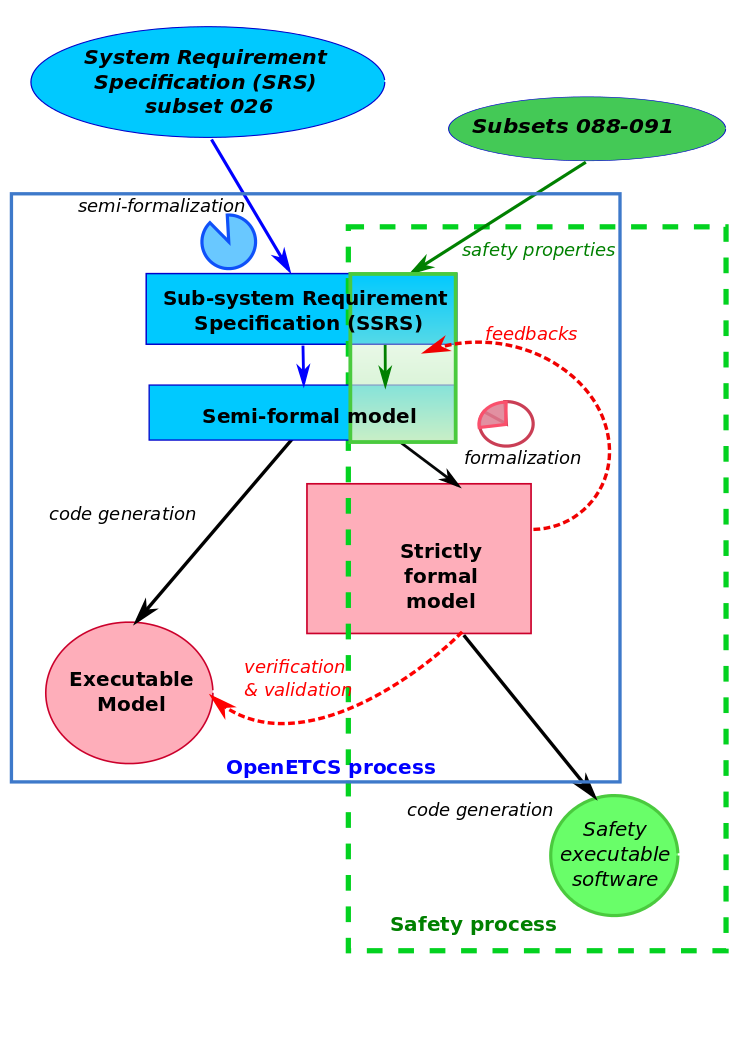
\includegraphics[width=4in]{OETCSProcess.png}}
  \caption{OpenETCS process}
  \label{fig:OETCSProcess}
\end{figure}


The proposed process for the OpenETCS project shall describe:
\begin{itemize}
\item how to design a semi-formal model of the on-board unit system from the SRS SUBSET-026 ;
\item how to design some subsets of the SRS SUBSET-026 within a safety process;
\item how to produce a running model of the application software of the on-board unit.
\end{itemize}

For the 2 first objectives, the semi-formal  model  shall take into account the safety constraints to apply to the design of a critical railway system.

The second part of this document describes the system to design during the OpenETCS project, as well as the scope of the safety activities on this system.

%%%%%%%%%%%%%%%%%%%%%%%%%%%%%%%%%%%%%%%%%%%%%%%%%%%%%%%%%%%%%%%

\section{Reference Documents}
\begin{itemize}
\item CENELEC EN 50126-1 --- 01/2000 --- \emph{Railways applications –- The specification and
demonstration of Reliability, Availability, Maintainability and Safety (RAMS) –- Part 1:
Basic requirements and generic process}
\item CENELEC EN 50128 --- 10/2011 --- \emph{Railway applications -- Communication, signalling and
processing systems -- Software for railway control and protection systems}
\item CENELEC EN 50129 --- 05/2003 --- \emph{Railway applications –- Communication, signalling and
processing systems –- Safety related electronic systems for signalling}
\item FPP --- \emph{Project Outline Full Project Proposal Annex OpenETCS} -- v2.2
\item SUBSET-026 3.3.0 --- \emph{System Requirement Specification}
\item SUBSET-076-x 2.3.y --- Test related ERTMS documentation
\item SUBSET-088 2.3.0 --- \emph{ETCS Application Levels 1 \& 2 - Safety Analysis}
\item SUBSET-091 3.2.0 --- \emph{Safety Requirements for the Technical Interoperability
of ETCS in Levels 1 \& 2}
\item CCS TSI --- \emph{ CCS TSI for HS and CR transeuropean rail has been adopted by a Commission Decision 2012/88/EU on the 25th January 2012}
\item D1.3 -- Project Quality Assurance Plan
\item D2.1 -- Report on existing methodologies 
\item D2.2 -- Report on CENELEC standards
\item D2.6 -- Requirements for OpenETCS
\end{itemize}

%%%%%%%%%%%%%%%%%%%%%%%%%%%%%%%%%%%%%%%%%%%%%%%%%%%%%%%%%%%%%%%

\section{Glossary}
\begin{description}
\item[API] Application Programming Interface
\item[FME(C)A] Failure Mode Effect (and Criticity) Analysis
\item[FIS] Functional Interface Specification
\item[HW] Hardware
\item[I/O] Input/Output
\item[OBU] On-Board Unit
\item[PHA] Preliminary Hazard Analysis
\item[QA] Quality Analysis
\item[RBC] Radio Block Center
\item[RTM] RunTime Model
\item[SIL] Safety Integrity Level
\item[SRS] System Requirement Specification
\item[SSHA] Sub-System Hazard Analysis
\item[SSRS] Sub-System Requirement Specification
\item[SW] Software
\item[THR] Tolerable Hazard Rate
\item[V\&V] Verification \& Validation
\end{description}




\section{OpenETCS Process}


\subsection{Overall Description}
\label{sec:overall_description}


To pursue the goals given in the introduction, the development cycle for the project is presented in this document.

The first objective of this process is to precisely defined, from the input documents, the \emph{sub-system} to design, ie. during this project the on-board unit of the ETCS system (see \ref{sec:casestudy}), and the needed elements to validate in safety this design.
In order to minimise the number of different models and to propose items which can be reused by railway actors after the end of the project, the proposed process shall take into account the safety concepts from the early steps, i.e., the sub-system requirement specification (SSRS) and the semi-formal definition of the model instead of the SRS. Thus, these elements can be used in the safety process to deduce formal models as shown in figure \ref{fig:OETCSProcess}.

The two most important elements of the System life-cycle of EN 50129 and the Software development life-cycle model of EN
50128 are the separation of the life-cycle into well-defined
phases and the focus on the production and recording of extensive documentation of the
development process. This allows facilitation of safety, verification, validation and assessment activities and confidence in the use of good practises to develop a critical system. To achieve this, an appropriate life-cycle
must be defined for OpenETCS, following the constraints provided by the CENELEC standard, and appropriate roles and responsibilities must be assigned to the participants.

 \begin{figure}
  \centering
  \fbox{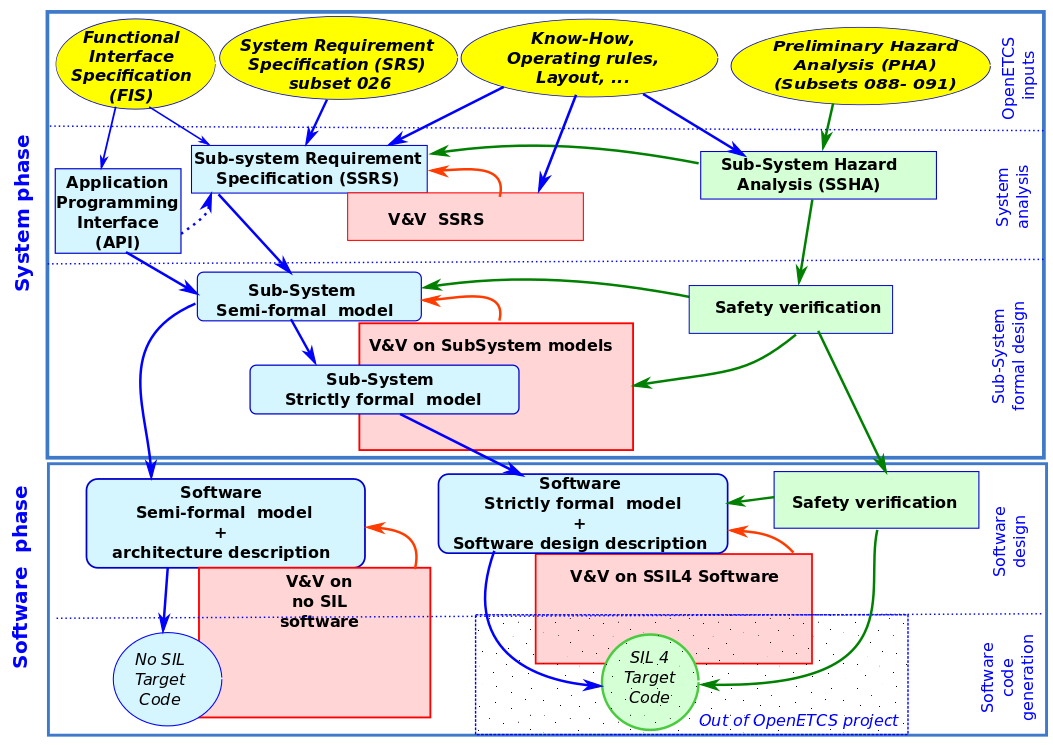
\includegraphics[scale=0.45]{WholeProcess.png}}
  \caption{Whole process}
  \label{fig:whole_process}
\end{figure}

Figure~\ref{fig:whole_process} describes the main phases and main activities of the OpenETCS process.
Input elements of the project are in yellow, specification and design activities in blue, verification and validation activities in red, safety activities in green.

Two main phases are defined :
\begin{description}
\item[System phase] to analyse the input documents and provide a model of the on
  board unit according to SUBSET-026 and the safety strategy:
\begin{itemize}
\item First, a system analysis (Step 1) shall provide a \textit{Sub-System Requirement Specification} (SSRS) to define the scope of the system to  design and its structure (activity a), completed with an abstract \textit{Application Programming Interface} (API) to  give the main interfaces of the system and interaction between software and hardware items (activity b). \textit{Sub-System Hazard Analyses} (SSHA) contains the safety analyses of the SSRS and  allows the definition of safety properties (activity d).
\item Second, a model (Step 2), at least semi-formal, is designed to describe sub-system
  architecture, main functions and to allocate sub-system requirements (activity a). This
  model will be completed with a formal model to focus on a subset of the
  functions or properties (activity b).
\end{itemize}
\item[Software phase] to design the software and then generate applicative code
  of the sub-system. Two approaches are developed in parallel from the same
  sub-system model:
\begin{itemize}
\item on one part to complete the semi-formal model (Step 3, activity a) to obtain a functional code covering as much as possible of the SSRS
\item on the other part to provide methods and tools to  obtain a SIL4 code and to apply this approach on a subset of the SSRS (Step 3 activity b).
\end{itemize}
\end{description} 

In the sequel, the main lines of this figure are going to be detailed. However, we are going to focus on specification and design activities only.

The Software Planning phase is defined by WP1 in the Quality Assurance Plan.
The Software Test / Validation phase is defined by WP4 in the Validation Plan.
The Software Verification activities are defined by WP4 in the Verification Plan.

Safety activities are described in EN50126.
The proof that the process satisfies the requirements of the standard is out of the scope of this document and shall be managed by the Safety Case (WP4).



%%%%%%%%%%%%%%%%%%%%%%%%%%%%%%%%%%%%%%%%%%%%%%%%%%%%

\subsection{Step 0: OpenETCS inputs}
\label{sec:inputs}


The main inputs of the OpenETCS project are the set of specifications provided by UNISIG as defined in annex A of CCS TSI. For the OpenETCS project, the initial reference is the baseline 3 (\url{http://www.era.europa.eu/Core-Activities/ERTMS/Pages/Current-Legal-Reference.aspx}). This reference baseline shall be modified only by project decision during a PCC meeting (see R-WP2/D2.6-02-044).
The main documents of this baseline for design activities are the \emph{System Requirement Specification} SUBSET-026~3.3.0 and the \textit{Functional Interface Specification} SUBSET-034-3.0.0.

These documents shall be completed with examples of national operating rules
provided by the railway operators such as Deutsche Bahn and SNCF, and with
know-how of the historical ERTMS manufacturers.



%%%%%%%%%%%%%%%%%%%%%%%%%%%%%%%%%%%%%%%%%%%%%%%%%%%%

\subsection{Step 1: System Analysis}
\label{sec:sys-analysis}


\subsubsection{Objectives}
\label{sec:sys-ana-objective}

The aim of this phase is to have a clear definition of the sub-system to design, which is not given by the input documents, and to define the scope of the model to design. Thus during this step, we shall identify:

\begin{itemize}
\item a set of requirements which describe the functionalities of the sub-system and the expected results concerning performance, maintainability, safety, reliability,...
\item the description of the architecture of the sub-system
\item the description of the external and internal interfaces of the sub-system.
\end{itemize}

Safety activities are necessary to define the safety requirements of the system and to define which functions are considered vital or non-vital respectively.

\subsubsection{Outputs}
\label{sec:sys-ana-outputs}

According to  design activities, two documents shall be produced during this phase :

\begin{description}
\item[Sub-System Requirement Specification (SSRS)] shall define the scope and the structure of the sub-system and  manage the requirement allocation on sub-systems and functions (see R-WP2/D2.6-02-45).
\item[Application Programming Interface (API)] shall describe the interfaces of the sub-system.
\end{description}


According to the CENELEC standards, these documents complete the input documents (SRS and FIS) to produce :
\begin{itemize}
\item the \emph{System  Requirements Specification} which describes all requirements of the system
\item the \emph{System Architecture Description
and Software / HW interface definition } which specify how the Software and the HW interact
as well as the location of the boundary between the two
\end{itemize}

\subsubsection{Detailed Description}
\label{sec:sys-ana-descr}

\paragraph{Activity a):SSRS definition} The first part is the definition of the  \emph{Sub System Requirement Specification} (SSRS) which shall allow:
\begin{itemize}
\item to clearly define the scope of SUBSET-026 to take into account the design (only on-board functionalities are designed, track-side functionalities are out of the scope of the project) (see R-WP2/D2.6-02-045.02.04),
\item to define the interfaces of the system: external interfaces and software/hardware interfaces (see WP2/D2.6-02-045.01, R-WP2/D2.6-02-045.02.05, R-WP2/D2.6-02-045.02.06),
\item to provide a functional architecture of the system with inputs and outputs of each function identified (see R-WP2/D2.6-02-045.02),
\item to allocate SRS requirements to each function and data-flow (see R-WP2/D2.6-02-045.03),
\item to classify Vital versus Non-Vital items (functions, input/output, requirements, ...) from the safety analysis results (see R-WP2/D2.6-02-046),
\end{itemize}

However, the SSRS shall be compliant with the input documents of TSI (SUBSET-026, FIS, ...) (see R-WP2/D2.6-02-045, R-WP2/D2.6-02-045.02.06 and R-WP2/D2.6-02-045.04) and shall cover all the requirements and the function of the input documents. If a function or a requirement shall not been taken into account in the sequel of the of the process, a justification shall be clearly given.

It shall also facilitate safety, design, verification, validation and maintenance activities: full traceability between SRS and SSRS shall be provided (see R-WP2/D2.6-02-045.05).

Detection of inconsistencies or ambiguities in the input documents shall be discussed and tracked (see R-WP2/D2.6-02-045.06).

These tasks need some interactions with safety activities, for example to define safety tags (ie; to precise if the artifacts are vital or not) on functions, requirements,...

\paragraph{Activity b): API definition} The second part is the definition of the \textit{Application Programming Interface} (API) : this document shall describe at an abstract level, how software and hardware parts of the sub-system are going to interact.
In particular, it will define an abstract layer of the hardware architecture (see R-WP2/D2.6-02-043), and a set of requirements on how the software is going to be executed in real time.

\subsubsection{Means and tools}

The SSRS and API shall be described as textual documents.
However these documents shall be completed by a semi-formal model to describe the functional architecture of the on-board unit (see R-WP2/D2.6-02-045.02.02):

\begin{itemize}
\item to  define the scope of the application to design (see R-WP2/D2.6-02-045.02.04),
\item to split the main function of the system into independent functions (see R-WP2/D2.6-02-045.02.01),
\item to describe the data flow between functions (see R-WP2/D2.6-02-045.02.03),
\item to describe the abstract interfaces of the sub-system and its environment, with respect to the existing input documents (see R-WP2/D2.6-02-045.02.05 and R-WP2/D2.6-02-045.02.06),
\item to  support allocation of the requirements to  the functions and data flow (see R-WP2/D2.6-02-045.03).
\end{itemize}

The requirements of the SRS are allocated to the
functions of the SSRS (the architecture), possibly split and rewritten in order to restrict their scope to these
functions. They are also rewritten in order to match the objects named in
the architecture (in particular internal and external I/O). The requirements are provided in natural language
(even if the objects are unambiguously named).

In view of verification activities, traceability between SSRS and SRS shall be provided (see R-WP2/D2.6-02-045.05). In practice, interpretations, additions and omissions of requirements shall be tracked and justified (see R-WP2/D2.6-02-045.05.01), as well as requirements exported to other sub-systems (see R-WP2/D2.6-02-045.05.02).

According to  CENELEC standards, no specific constraints are given on the tools used during this step: textual and graphical editors, with syntax checker, are needed to  produce documents and models. Tools classified as T1 according EN50128 can be used.

%%%%%%%%%%%%%%%%%%%%%%%%%%%%%%%%%%%%%%%%%%%%%%%%%%%%

\subsection{Step 2: Sub-System formal design}
\label{sec:subsyst-formal-design}



\subsubsection{Objectives}
\label{sec:sys-fm-objective}

The aim of this phase is to provide a model of the sub-system from the SSRS:

\begin{itemize}
\item to provide a semi-formal reference specification of the sub-system requirements
\item to lift ambiguities
\item to detect errors and inconsistencies.
\end{itemize}


\subsubsection{Outputs}
\label{sec:sys-fm-outputs}


The main output of this step is a \textit{semi-formal model of the sub-system}  covering the architecture, interface description and requirement allocation of the SSRS.

This semi-formal model can be extended with \textit{strictly formal models} to improve the understanding of the sub-system and to provide elements for verification and validation activities.

\subsubsection{Detailed Description}
\label{sec:sys-dev-deta-descr}


\paragraph{Activity a): Sub-system semi-formal modeling} To cover the OpenETCS project objective  of formal models, a semi-formal model of the system  specification is defined from  the SSRS (see R-WP2/D2.6-02-047). This model shall reflect the architecture defined in SSRS (see R-WP2/D2.6-02-045.02.02). Requirements of the sub-system can be refined in semi-formal means but the semi-formal model  shall be as consistent as possible with the SSRS level of abstraction (see R-WP2/D2.6-02-047.02), in particular choices concerning software architecture and design have not to be described at this level.
In practice, all the requirements of SSRS (see R-WP2/D2.6-02-047.02.01) and of the sub-system Hazard analysis (see R-WP2/D2.6-02-047.02.02) shall be covered by the semi-formal model.

Traceability between semi-formal model and SSRS shall be provided (see R-WP2/D2.6-02-047.02.05): interpretations, additions and omissions of requirements shall be tracked and justified (see R-WP2/D2.6-02-047.02.03), as well as exported requirements  (see R-WP2/D2.6-02-047.02.06).

\paragraph{Activity b): Sub-system strictly formal modeling} This semi-formal model can be extended with strictly formal models to improve the understanding of some part of the sub-system (see R-WP2/D2.6-02-049) and to  provide elements for verification and validation activities especially concerning safety properties.

To facilitate safety activities, the safety relevant function should be as much as possible insulated from non safety relevant functions (see R-WP2/D2.6-02-052).

Traceability between strictly formal model and semi-formal model shall be provided (see R-WP2/D2.6-02-049.03): interpretations, additions and omissions of requirements shall be tracked and justified (see R-WP2/D2.6-02-049.03.01), on the sub-parts to model only.

\subsubsection{Means and tools}

The means of description of the semi-formal model shall be understandable by domain experts (see R-WP2/D2.6-02-065), providing graphical  description (see R-WP2/D2.6-02-065.01).

The semi-formal model shall reflect the functional architecture defined in SSRS. In particular the language used to  design the semi-formal model shall allow it to be modular and extensible (see R-WP2/D2.6-02-050).

In view of validation activities, the means of description of the semi-formal model shall allow to simulate it (see R-WP2/D2.6-02-048 and R-WP2/D2.6-02-071).

Parts of the sub-system shall be modelled strictly formally (see R-WP2/D2.6-02-049). This formal model shall be derived from the semi-formal one (see R-WP2/D2.6-02-049.02), as straightforward and automated as possible (see R-WP2/D2.6-02-049.05). Thus, the semi-formal model shall be designed (language and structure) in order to allow the design and validation of the strictly formal model (see R-WP2/D2.6-02-049.04); and to be easily translatable to other languages (see R-WP2/D2.6-02-068).
As for semi-formal model, the strictly formal model shall be modular and extensible (see R-WP2/D2.6-02-051) and shall refine the modular design of the semi-formal model (see R-WP2/D2.6-02-051.01).


The expressiveness of the language used to design the semi-formal and formal models shall allow formalisation of the classical objects used in the description of critical systems (see R-WP2/D2.6-02-069 and R-WP2/D2.6-02-070):

\begin{itemize}
\item state machines
\item time-outs
\item truth tables
\item arithmetics
\item braking curves
\item logical statements
\item messages and fields
\end{itemize}


In view of safety activities, the languages used for the models shall allow a declarative and formal expression of the safety properties (see R-WP2/D2.6-02-066), understandable by domain experts (see R-WP2/D2.6-02-066.01). The modelled safety properties shall be validated on the semi-formal model by test and on the strictly formal model by proof (see R-WP2/D2.6-02-058). Logical assertion can be added to simplify the models but shall be validated just as the properties or requirements (see R-WP2/D2.6-02-072).

All means of description used shall be standardised or at least documented in detail (see R-WP2/D2.6-02-067). 

According to  CENELEC standards, no specific constraints are given on the tools used during this modelling step: textual and graphical editors, with syntax checker, are needed to  produce documents and model. Tools classified as T1 according EN50128 can be used.


%%%%%%%%%%%%%%%%%%%%%%%%%%%%%%%%%%%%%%%%%%%%%%%%%%%%

\subsection{Step  3: Software design}
\label{sec:sw-design}

\subsubsection{Objectives:}
\label{sec:sw-req-objective}


In this phase, the system requirements shall be refined to take into account software constraints.

Two branches are considered:
\begin{itemize}
\item  The aim of the first branch  is to  design all the functionalities of the SSRS to  produce functional code, without SIL. As much as possible of the requirements of the SSRS shall be covered in this phase.
\item The aim  of the second branch is to provide a method and a toolchain to produce SIL 4 code. This approach has to be evaluated on a subset of the SSRS requirements.
\end{itemize}


\begin{figure}[h]
  \centering
  \fbox{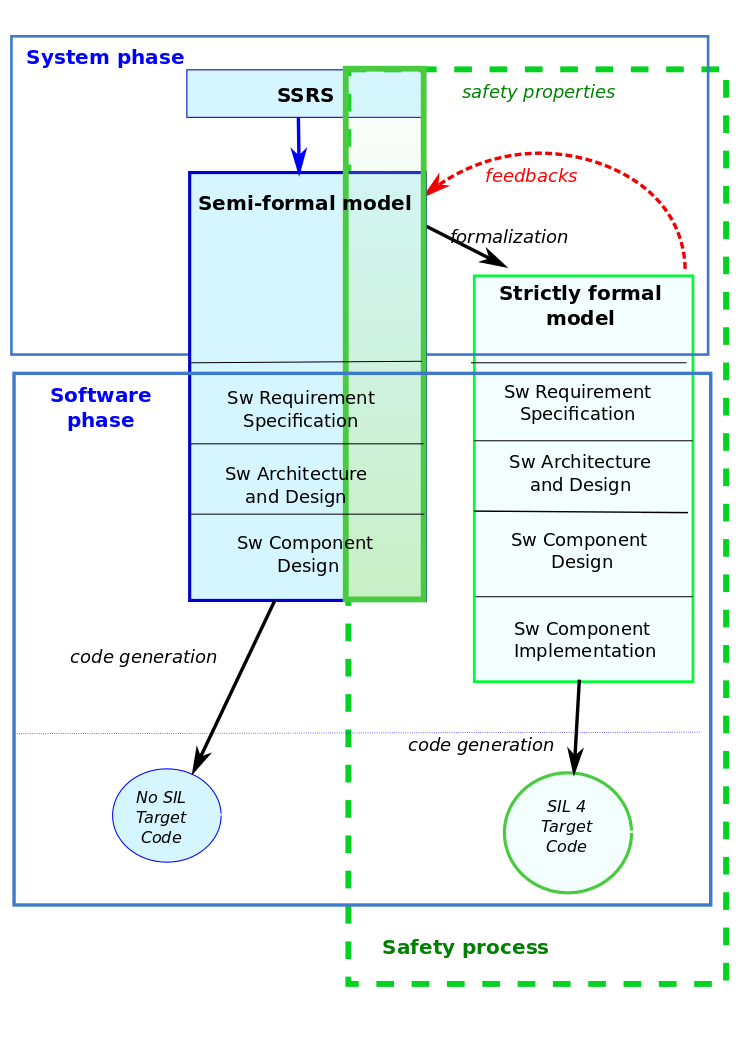
\includegraphics[width=4in]{Model-phase.png}}
  \caption{Software phase description}
  \label{fig:detailed software}
\end{figure}


\subsubsection{Activity a): Functional branch}
\label{sec:sw-func}

For this branch, the semi-formal model  defined during the system phase, shall  be completed and detailed with software constraints in such a way that it is possible to produce executable code for a given target.


\paragraph{Outputs:}
\label{sec:sw-func_out}

The main output of this step  is a semi-formal model which  allows to produce executable code.
This model  shall be completed by a \textit{Software Architecture and Design Specification}, which describes the software architecture and the design choices.


\paragraph{Detailed Description:}
\label{sec:sw-req-deta-descr}

Taking into account the SSRS requirements allocated to  the software, a software architecture shall be defined, with a description of all the input/output of the software, as well as a description of the operational modes and behaviour.

Then, each software component is designed according to  the sub-system  requirements: All sub-system requirements allocated to  software shall be referenced in the model or a justification shall be given.

It shall provide all the elements to have testable requirements on a target platform. All functions to perform shall be clearly identified. Defined interfaces (internal and external) shall be  taken into account.


\paragraph{Means and tools}
\label{sec:sw-means}

The semi-formal model defined during the system phase shall be completed, keeping the same language or extending it to  cover specific software aspects.

The model  shall be at least semi-formal, however, strictly  formal  methods could be necessary for single activities.

\subsubsection{Activity b): Functional and safety branch}

For this branch, we shall provide methods and a toolchain to  obtain SIL4 executable code of the on-board software application. 

Thus, the software design activities shall be consistent with the three software development phases according EN 50128 :

\begin{itemize}
\item Software Requirements Phase
\item Software Architecture and Design Phase
\item Software Component Design Phase
\end{itemize}

\paragraph{Outputs:}
\label{sec:sw-req-documents}
From a design point of view, the outputs to produce in this phase are:

\begin{itemize}
\item a formal model of the software including the software requirements, the software architecture and the software component design
\item  a document  \textit{Software Architecture and Design} to  detail software architecture and design choices.
\end{itemize}


\paragraph{Detailed Description:}
\label{sec:sw-req-deta-descr}

The first step of this phase is to give an explicit description of software requirements according to system requirements and safety properties.  Then, a software architecture shall be proposed according to software design choices detailed in  \textit{Software Architecture and Design}.
Finally, each software component shall be modelled in detail.

The method and process used during this activities shall cover the constraints of sections 7.2, 7.3 and 7.4 of EN 50128 or justification shall be given.


However this model takes care of the following :

\begin{itemize}
\item It shall give a description of all the input/output of the software, as well as a description of the operational modes and behaviour (cf. §7.2.4.5,  §7.2.4.6 and  §7.2.4.7 of EN 50128). 
\item It shall provide all the elements to have testable requirements on a target platform. All functions to perform shall be clearly identified. (cf. §7.2.4.4, §7.3.4.5  of EN 50128).
\item All existing constraints between hardware and software will be taken into account (cf. §7.2.4.9, §7.3.4.4 and §7.3.4.5 of EN 50128).
\item It shall be developed in a way which allows meeting the software
requirements and the necessary safety requirements without introducing
unnecessary complexity (cf. §7.2.4.3,  §7.2.4.4  of EN 50128).
\item There shall also be an evaluation of the
Hardware / Software interaction, its influence on the safety aspects of the system and the
evaluation of the usage of already existing software  (cf. §7.2.4.10,  §7.2.4.12 and §7.2.4.13  of EN 50128).
\item It shall give a  description of the design choices, in particular software component decomposition, data description and requirement allocations (cf. §7.3.1 of EN 50128).
\end{itemize}

For the OpenETCS project, at least methods and toolchain shall be provided and evaluated on a subset of the SSRS.

\paragraph{Means and tools}
\label{sec:sw-means}

Definition of a strictly formal  model is highly recommended by EN 50128, and should be derived from  the system  model.


Selected tools for this activities shall  be of class T1 or T2  depending how they deal  with verification and validation activities.

%%%%%%%%%%%%%%%%%%%%%%%%%%%%%%%%%%%%%%%%%%%%%%%%%%%%

\subsection{Step 4: Software code generation}
\label{sec:sw-code}



\subsubsection{Objectives:}
\label{sec:sw-req-objective}


In this phase, software code is produced from the software models.

\subsubsection{Activity a): Demonstrator}
\label{sec:demo-phase}

A first executable code is produced from the software functional model (see R-WP2/D2.6-02-086). This executable code shall be non vital (see R-WP2/D2.6-02-087). However it shall be able to run in real time (see R-WP2/D2.6-02-088) on a on-board computer (see R-WP2/D2.6-02-090).
Thus it shall comply to the standardised interfaces (see R-WP2/D2.6-02-089). 

There are no specific constraints on the means and tools to  produce this non SIL code.

%%%%%%%%%%%%%%%%%%%%

\subsubsection{Activity b): SIL4 Code}
\label{sec:code-phase}

During this phase code should be produce in safety from the safety functional model.

This code cannot be provided by the OpenETCS project : Safety  activities are not conducted in the whole scope of the on-board unit sub-system, and elements of the target platform are not provided.

However, the description of how to  produce such a code in a safe way is part of the OpenETCS project. This corresponds to the lower phases of the process according to  E50128 :
\begin{itemize}
\item Software Component Implementation Phase
\item Integration
\end{itemize}


\paragraph{Means and tools}
\label{sec:code-means}

Proposal shall include methods and tools covering criteria of § 7.5 and §6.7 of EN 50128.
If an automatic generation of the code from the formal model is proposed, the tool in charge of this generation shall cover criteria of T3 tools.


%%%%%%%%%%%%%%%%%%%%%%%%%%%%%%%%%%%%%%%%%%%%%%%%%%%%





\section{OpenETCS Case Study}
\label{sec:casestudy}



The EVC (European Vital Computer) is the heart of the ERTMS on-board system. This safety relevant
computer implements the functions of the SRS subset 026 of UNISIG (for SRS versions beginning
with baseline 3, published by ERA) in order to guarantee the safety of the train movements.
The OpenETCS scope of application is related only to the EVC part of whole ERTMS system.
The track-side part of the ETCS (the Radio Based Control) is excluded from the project activities, it is
only considered through its interfaces with the on-board part of ETCS.

A detailed specification of the sub-system will be given during the system analysis phase: the Sub-System Requirement Specification shall contain 
\begin{itemize}
\item the high level description of the openETCS case study
\item the environment and the architecture of the sub-system  to design, with
  interfaces of the main functions and data-flows
\end{itemize}

Safety properties shall be given in the sub-system hazard analysis.





%%%%%%%%%%%%%%%%%%%%%%%%%%%

%% Bibliography
\nocite{*}
\bibliographystyle{unsrt}
\bibliography{erdc}
\bibliography{process}



% \begin{thebibliography}{9}

% \bibitem{lamport94}
  % Leslie Lamport,
  % \emph{\LaTeX: A Document Preparation System}.
  % Addison Wesley, Massachusetts,
  % 2nd Edition,
  % 1994.

% \end{thebibliography}

%===================================================
%Do NOT change anything below this line

\end{document}
